\documentclass[11pt]{article}
\usepackage[sc]{mathpazo}
\usepackage{amsmath}
\usepackage{fullpage}
\usepackage[authoryear,sectionbib,sort]{natbib}
\linespread{1.7}
\usepackage[utf8]{inputenc}
\usepackage{lineno}

\usepackage{graphicx} 
%\usepackage{a4wide}
%\usepackage{multicol,caption}
%\setlength{\textwidth}{16cm}
%\setlength{\textheight}{22cm}

\title{Density-dependent selection in evolutionary genetics: a lottery model of Grime's triangle}
\author{Jason Bertram $^{1,\ast}$ \\ 
Joanna Masel $^{1}$}

\date{}

\begin{document}

\maketitle

\noindent{}1. Department of Ecology and Evolutionary Biology, University of Arizona, Tucson, AZ 85721.

\noindent{}$\ast$ Corresponding author; e-mail: amnat@uchicago.edu.


\bigskip

\textit{Manuscript elements}: Figure~1, figure~2, table~1, online
appendices~A and B (including figure~A1 and figure~A2). Figure~2 is to
print in color.

\bigskip

\textit{Keywords}: Examples, model, template, guidelines.

\bigskip

\textit{Manuscript type}: Article. 
% Or e-article, note, e-note, natural history miscellany,
% e-natural history miscellany, comment, reply, symposium, or
% countdown to 150.

\bigskip

\noindent{\footnotesize Prepared using the suggested \LaTeX{} 
template for \textit{Am.\ Nat.}}

\linenumbers{}
\modulolinenumbers[3]

\newpage{}

\section*{Abstract}

The classic lottery model is generalized to accomodate arbitrary densities. We use the model to predict the direction of trait evolution under different environmental conditions and thereby provide a mathematical underpinning for Grime's verbal theory of plant primary strategies. We evaluate the density-dependent lottery model as a general-purpose model of density-dependent selection in the spirit of MacArthur's $r$/$K$ theory. 

\newpage{}

``...the concept of fitness is probably too complex to allow of a useful mathematical development. Since it enters fundamentally into many population genetics considerations, it is remarkable how little attention has been paid to it.'' --- Warren J. Ewens, Mathematical Population Genetics I, 2004 

\section*{Introduction}

Evolutionary models differ greatly in their treatment of fitness. In models of genetic evolution, genotypes are typically assigned constant (or frequency-dependent) selection coefficients describing the change in their relative frequencies over time due to differences in viability. This considerably simplifies the mathematics of selection, facilitating greater genetic realism, and can be justified over sufficiently short time intervals \citep[p. 276]{ewens_2012}. However, selection can have very different effects when operating on different types of traits, and evolutionary changes in one population can lead to complicated ecological responses.

By contrast, models of phenotypic trait evolution represent the change in phenotypic abundances over time using absolute fitness functions which describe how those traits affect survival and reproduction in particular ecological scenarios. This approach is powerful enough to model eco-evolutionary feedbacks between co-evolving traits, but is generally problem-specific and restricted to only a few traits at a time.

Far less work has been done to model fitness in more general terms than particular traits or ecological scenarios, while still capturing key distinctions between different forms of selection. Perhaps this is not surprising given that fitness is such a complex quantity, dependent on all of a phenotype's functional traits \citep{violle_2007} as well as its biotic and abiotic environment. In most cases, a detailed, trait-based, predictive model of fitness would be enormously complicated and have narrow applicability. It is therefore easy to doubt the feasibility of a simplified, general mathematical treatment of fitness \citep[p. 276]{ewens_2012}. Even MacArthur's famous r/K selection scheme is now almost exclusively known as a framework for understanding life-history traits, and judged on its failure in that role \citep{pianka_1970,stearns_1977,boyce_1984,reznick_2002}. In spite of the r/K scheme's original purpose as an extension of the existing population-genetic treatment of selection to account for population density \citep{macarthur_1962}, comparatively few attempts have been made to develop it further as a mathematical analysis of the major different forms of selection. 

Nevertheless, there are strong indications there are broader principles governing the operation of selection. In many groups of organisms, including corals \citep{darling_2012}, insects \citep{southwood_1977}, fishes \citep{winemiller_1992}, zooplankton \citep{allan_76} and plants \citep{grime_1988,westoby_1998}, different species can be divided into a small number of distinct trait clusters corresponding to fundamentally distinct ``primary strategies'' \citep{winemiller_2015}. The most famous example is Grime's plant trait classification scheme \citep{grime_1974,grime_1977,grime_1988}. Grime considered two broad determinants of population density: stress (persistent hardship e.g. due to resource scarcity, unfavorable temperatures or toxins) and disturbance (intermittent destruction of vegetation e.g. due to trampling, herbivory, pathogens, extreme weather or fire).  The extremes of these two factors define three primary strategies denoted by C/S/R respectively: competitors ``C'' excel in low stress, low disturbance environments; stress tolerators ``S'' excel in high stress, low disturbance environments; and ruderals ``R''  excel in low stress, high disturbance environments. Survival is not possible in high-stress, high-disturbance environments. Grime showed that measures of C, S and R across a wide range of plant species are anti-correlated, so that strong C-strategists are weak S and R strategists, and so on. Thus, plant species can be classified on a triangular C/S/R ternary plot \citep{grime_1974}. Trait classification schemes for other organisms are broadly analogous to Grime's scheme \citep{winemiller_2015}. 

Trait classification schemes show empirically that, beneath the complicated details of trait variation, even among closely-related species, fitness is predominantly determined by a few key factors such as intrinsic reproducive rate or stress-tolerance. However, while trait classification schemes are firmly grounded in trait data, they are verbal and descriptive rather than mathematical, a recognized hinderance to their broader applicability (e.g. \citep{tilman_2007}). 

The aim of this paper is explore the interplay between some major dimensions of fitness in a simplified, spatially-homogeneous model of genotype growth, dispersal and competition. Building on the earlier r/K and C/S/R schemes, a central question is how fitness depends on the interaction between population density, intrinsic birth/death rates and competitive ability. 

We broadly follow the spirit of MacArthur's $r$/$K$ selection scheme in that our model is intended to account for fundamentally different forms of selection without getting  entangled in the intricacies of particular ecological scenarios. However, rather than building directly on MacArthur's formalism and its later extensions using Lotka-Volterra equations to incorporate competition (``$\alpha$-selection'') \citep{gill_1974,case_1974,joshi_2001}, our model is devised primarily with Grime's C/S/R scheme in mind, and represents a quantitative formalization of how C/S/R manifests at the level of genotype evolution (as opposed to divergence between species). This choice is motivated in part by the substantial empirical support for the C/S/R scheme, and in part by the failings of the $r$/$K$ low/high density dichotomy --- many growth ability traits will confer advantages at both low and high densities (more details in the Discussion). 

In section ``Model'' we introduce the basic assumptions of our generalized lottery model. Analytical expressions for the change in genotype abundances over time are introduced in section ``Mean field approximation'', with mathematical details relegated to the Appendices. The following two sections discuss the behaviour of rare mutants and our treatment of Grime's triangle. 
 

\section*{Model}\label{sec:model}

We assume that each individual in a population requires its own territory to survive and reproduce (a site-occupancy model). All territories are identical, and the total number of territories is $T$. Time $t$ advances in discrete iterations, each representing the average time from birth to reproductive maturity. In iteration $t$, the number of reproductively mature individuals (henceforth called ``adults'') of the $i$'th genotype is $n_i(t)$, the total number of adults is $N(t)=\sum_i n_i(t)$, and the number of unoccupied territories is $U(t)=T-N(t)$. 

Each iteration, adults produce $m_i$ new offspring (henceforth called ``propagules'') which disperse at random over the $U$ unnocupied territories (no dispersal limitation). We assume adults cannot be ousted from occupied territories, so only propagules landing on occupied territories are included in $m_i$. More generally, $m_i$ does not include propagules which never even begin the development cycle. For simplicity, we assume $m_i=b_i n_i$, where $b_i$ is a constant, genotype-specific birth rate. 

The number of individuals of the $i$'th genotype landing in any particular territory is denoted $x_i$. Random dispersal implies that in the limit $K\rightarrow \infty$, with $n_i/K$ held fixed, $x_i$ is Poisson distributed with mean territorial propagule density $l_i=m_i/U$. Although $T$ is finite in our model, we assume that $K$ and the $n_i$ are large enough that $x_i$ is Poisson-distributed to a good approximation (details in Appendix A). This dispersal Poisson distribution is denoted $p_i(x_i)$. Note that the large $n_i$, large $T$ approximation places no restrictions on our densities $n_i/T$, but it does preclude consideration of demographic stochasticity when $n_i$ itself is very small (this will be discussed further in Section \ref{sec:invas}).

When multiple propagules land on the same territory, they compete to secure the territory as they develop. This territorial contest is modeled as a weighted lottery: the probability that genotype $i$ wins a given territory by the next iteration is $c_i x_i/\sum_j c_j x_j$ where $c_i$ is a constant representing relative competitive ability. 

The increase in $n_i$ over one iteration due to territorial acquisition, $\Delta_+ n_i$, is the sum of genotype $i$'s victories over all $U$ unoccupied territories. Since $p_1(x_1)\ldots p_G(x_G)$ is equal to the proportion of unoccupied territories with $x_1,\ldots,x_G$ of the respective propagules (again, we assume that $T$ is large enough that fluctuations in this proportion are negligible), this sum can be replaced by an expectation over the $p_i$. This gives
\begin{equation}
\Delta_+ n_i(t)=U(t)\sum_{x_1,\ldots,x_G} \frac{c_i x_i}{\sum_j c_j x_j} p_1(x_1)\ldots p_G(x_G). \label{eq:growthsumuncoupled}
\end{equation}

In addition to propagule birth and competition, occupied territories become unoccupied due to mortality. For the vast majority of this manuscript we assume that mortality only occurs in adults, and at a constant, genotype-specific per-capita rate $d_i$, so that the overall change in genotype abundances is
\begin{equation}
\Delta n_i(t)=\Delta_+ n_i(t)-d_i n_i(t). \label{eq:delttot}
\end{equation}
We will introduce a different mortality model when we consider the effects of disturbances (Section \ref{sec:grime}), which will also affect competing juveniles. 

Note that the competitive ability coefficients $c_i$ represent a strictly relative aspect of fitness in the sense that they only influence population size $N$ indirectly by changing genotype frequencies; that may in turn change the population mean birth and death rates. This can be seen by summing Eq. \eqref{eq:delttot} over genotypes to get the  change in population size $N$, 
\begin{equation}
\Delta N=U(1-e^{-L})-\sum_i d_i n_i,\label{eq:deltN}
\end{equation}
which is independent of $c_i$ (here $L=\sum_j l_j$ is the overall propagule density).

\section*{Results}

\subsection*{Mean Field Approximation}

Eq. \eqref{eq:delttot} gives little intuition about the dynamics of density-dependent lottery competition, since \eqref{eq:growthsumuncoupled} involves an expectation over the random dispersal distributions $p_i$, which depend on how the $n_i$ change over time. We now evaluate this expectation using a ``mean field'' approximation; the intuition behind this approximation is as follows.

If the unoccupied territories are saturated with propagules from every genotype ($l_i\gg 1$ for all genotypes), the fluctuations in the $x_i$ are small compared to their means $l_i$ (since the $x_i$ are Poisson distributed), and so the composition of propagules in a territory will only rarely differ appreciably from the mean composition $l_1,l_2,\ldots,l_G$. Consequently, we can replace $x_i$ with $l_i$ in Eq. \eqref{eq:growthsumuncoupled}. This gives the classic lottery model \citep{chesson_1981},
\begin{equation}
\Delta_+ n_i(t)=U(t)\frac{c_i m_i}{\sum_j c_j m_j}= b_i n_i\frac{1}{L}\frac{c_i}{\overline{c}}, \label{eq:lottery}
\end{equation}
where $\overline{c}=\sum_j c_j m_j/M$ is the mean propagule competitive ability for a randomly selected propagule ($M=\sum_j m_j$ is the total number of propagules). 

However, in general the $l_i$ are not all large, and the $x_i$ cannot simply be replaced by their means in Eq. \eqref{eq:growthsumuncoupled}. Indeed, Eq. \eqref{eq:lottery} is nonsensical if $l_i$ is sufficiently small: genotype $i$ can win at most $m_i$ territories, yet Eq. \eqref{eq:lottery} demands a fraction $c_i m_i/\sum_j c_j m_j$ of the unoccupied territories $U$, no matter how large $U$ is. The source of this pathological behavior when $l_i\ll 1$ is that $x_i=1$ in the few territories where $i$ propagules do land, and so $i$'s growth comes entirely from territories which deviate appreciably from the mean.  

Our mean field approximation is similar to the high-$l_i$ approximation leading to Eq. \eqref{eq:lottery} in that we replace the $x_i$ with appropriate mean values. The key distinction is that territories with a single propagule from the focal genotype, which are critical at low densities, are handled separately. In place of the requirement of $l_i\gg 1$ for all $i$, our approximation only requires that there are no large discrepancies in competitive ability (specifically, that we do not have $c_i/c_j\gg 1$ for any two genotypes; further discussion in section ``Discussion''). We obtain (details in Appendix B)
\begin{equation}
\Delta_+ n_i(t)\approx b_i n_i\left[e^{-L}+(R_i+A_i)\frac{c_i}{\overline{c}}\right], \label{eq:master}
\end{equation}
where
\begin{equation}
R_i=\frac{\overline{c}e^{-l_i}(1-e^{-(L-l_i)})}{c_i +\frac{L-1+e^{-L}}{1-(1+L)e^{-L}}\frac{\overline{c}L- c_il_i}{L-l_i}},\label{eq:Dr}
\end{equation}
and
\begin{equation}
A_i=\frac{\overline{c}(1-e^{-l_i})}{c_il_i\frac{1-e^{-l_i}}{1-(1+l_i)e^{-l_i}}+\sum_{j\neq i}\frac{c_jl_j}{L-l_j}\left(L\frac{1-e^{-L}}{1-(1+L)e^{-L}}-l_j\frac{1-e^{-l_j}}{1-(1+l_j)e^{-l_j}}\right)}.\label{eq:Da}
\end{equation}

Comparing Eq. \eqref{eq:master} to Eq. \eqref{eq:lottery}, the classic lottery per-propagule success rate $c_i/\overline{c}L$ has been replaced by three separate terms. The first, $e^{-L}$, accounts for propagules which land alone on unoccupied territories; these territories are won without contest. The second term, $R_i c_i/\overline{c}$ represents competitive victories when the $i$ genotype is a rare invader in a high density population: from Eq. \eqref{eq:Dr}, $R_i\rightarrow 0$ when the $i$ genotype is abundant ($l_i\gg 1$), or other genotypes are collectively rare ($L-l_i\ll 1$). The third term, $A_ic_i/\overline{c}$, represents competitive victories when the $i$ genotype is abundant: $A_i\rightarrow 0$ if $l_i\ll 1$. The relative importance of these three terms varies with both the overall propagule density $L$ and the relative propagule frequencies $l_i/L$. If $l_i\gg 1$ for all genotypes, we recover the classic lottery model (only the $A_ic_i/\overline{c}$ term remains, and $A_i\rightarrow 1/L$). Thus, Eq. \eqref{eq:master} generalizes the classic lottery model to account for arbitrary propagule densities for each genotype. 

Fig.~\ref{fig:simcomp} shows that Eq. \eqref{eq:master} (and its components) closely approximate direct simulations of random dispersal and lottery competition over a wide range of propagule densities (obtained by varying $U$). Two genotypes are present, one of which has a $c$-advantage and is at low frequency. The growth of the low-frequency genotype relies crucially on the low-density competition term $R_i c_i/\overline{c}$, and also to a lesser extent on the high density competition term $A_i c_i/\overline{c}$ if $l_1$ is large enough (Fig.~\ref{fig:simcomp}b). On the other hand, $R_i c_i/\overline{c}$ is negligible for the high-frequency genotype, which depends instead on high density territorial victories (Fig.~\ref{fig:simcomp}d). 

\begin{figure}
\centering
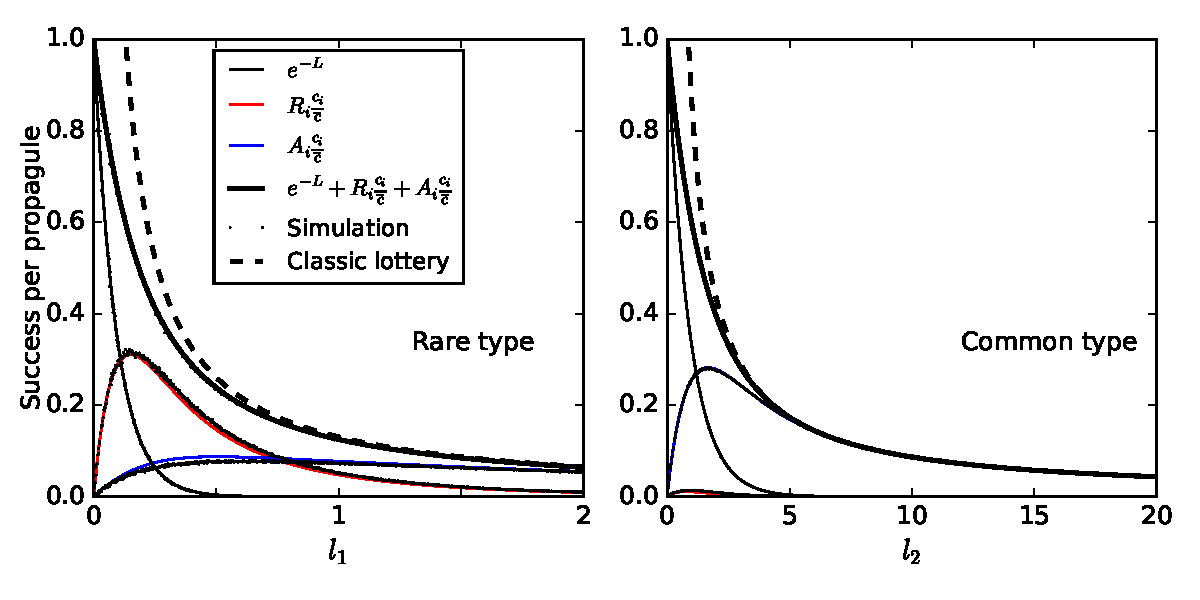
\includegraphics[scale=0.7]{simulationcomparison.pdf}
\caption{\label{fig:simcomp} The change in genotype abundances in a density dependent lottery model is closely approximated by Eq. \eqref{eq:master}. $\Delta_+ n_i/m_i$ from Eq. \eqref{eq:master} (and its separate components) are shown, along with direct simulations of random dispersal and lottery competition over one iteration over a range of propagule densities (varied by changing $U$ with the $m_i$ fixed). Two genotypes are present. (a) and (b) show low-frequency genotype with $c$-advantage ($m_1/M=0.1$, $c_1=1.5$), (c) and (d) show the high-frequency predominant genotype ($m_2/M=0.9$, $c_2=1$).} 
\end{figure}

%with the exception of large discrepancies in competitive ability since it is extremely unlikely that a large discrepancy competitive would arise in the absence of migration. 

\subsection*{Invasion of rare genotypes and coexistence}\label{sec:invas}

To determine how $b$, $c$ and $d$ will evolve in a population where those traits are being modified by mutations, we need to know whether mutant lineages will grow (or decline) starting from low densities. In this section we discuss the behavior of rare genotypes predicted by Eq. \eqref{eq:master}. 

Suppose that a population with a single genotype $i$ is in equilibrium. Then $R_i=0$, $\overline{c}=c_i$ and $\Delta n_i = 0$, and so Eq. \eqref{eq:master} gives
\begin{equation}
b_i\left(e^{-L}+A_i\right)-d_i=0.\label{eq:equil}
\end{equation}
Now suppose that a new genotype $j$, which is initially rare, appears in the population. Then $A_j\ll 1$, $l_j\ll L$ and $\overline{c}\approx c_i$, and so, from Eq. \eqref{eq:master}, $n_j$ will increase if 
\begin{equation}
b_j \left(e^{-L}+R_j\frac{c_j}{c_i}\right)-d_j>0.\label{eq:invad}
\end{equation}

Combining Eqs. \eqref{eq:equil} and \eqref{eq:invad}, it is easily verified that if $j$ is superior in one trait, but otherwise identical to $i$, it will invade. Moreover, $j$ will eventually exclude $i$, since it is strictly superior. However, stable coexistence is possible between genotypes that are superior in different traits. To illustrate, suppose that $j$ is better at securing territories ($c_j>c_i$), that $i$ is better at producing propagules ($b_i>b_j$), and that $d_i=d_j$. Coexistence occurs if $j$ will invade an $i$-dominated population, but $i$ will also invade a $j$-dominated population (``mutual invasion''). It is not hard to show that this is possible, since if $b_i$ is so large that $L\gg 1$ when $i$ is dominant, and $b_j$ is so small that $L\ll 1$ when $j$ is dominant, then, combining Eqs. \eqref{eq:equil} and \eqref{eq:invad}, we find that $i$ invades $j$ because $b_i>b_j$, while $j$ invades $i$ provided that
\begin{equation}
b_jc_jR_j-b_i c_i A_i>0. \label{eq:jinvadcoex}
\end{equation}
Thus, coexistence occurs if $c_j$ is large enough. Intuitively, the mechanism for coexistence is that territorial contests are important in an $i$-dominated population (high $L$), ensuring that the $c$-specialist $j$ is not excluded, yet territorial contests are irrelevant in a $j$-dominated population (low $L$), ensuring that the $b$-specialist $i$ is not excluded. Fig.~\ref{fig:coex} shows an example of this coexistence between $b$ and $c$ specialists. 

\begin{figure}
\centering
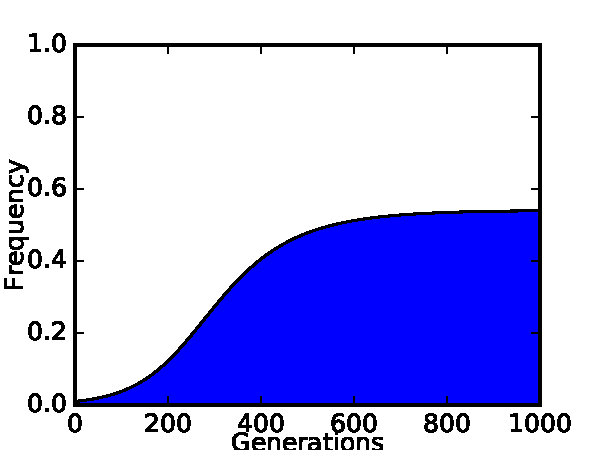
\includegraphics[scale=0.7]{coex.pdf}
\caption{\label{fig:coex} Coexistence between $b$ ($c_i=1$, $b_i=1$) and $c$ ($c_j=2$, $b_j=0.7$) specialists, where $d_i=d_j=0.3$. Vertical axis shows frequency of the $c$-specialist predicted by Eq. \eqref{eq:master}.} 
\end{figure}

A similar argument applies for coexistence between high-$c$ and low-$d$ specialists; again coexistence occurs because the importance of territorial contests declines along with propagule density $L$ as the $c$-specialist increases in frequency. Coexistence is technically possible between $b$- and $d$-specialists which exactly satisfy $b_i/d_i=b_j/d_j$ (this follows from the fact that all propagules have the same probability of success when $c_i=c_j$ i.e. $A_i+R_i=A_j+R_j$). However, this coexistence scenario is not biologically relevant, since the tiniest deviation from $b_i/d_i=b_j/d_j$ will lead to the eventual exclusion of the genotype with greater $b_i/d_i$. 

If the rare genotype $j$ arises due to mutation, then it's initial low-density behavior is more complicated than the above invasion analysis suggests. The mutant lineage starts with one individual $n_j=1$, and remains at low abundance for many generations after its initial appearance. During this period, the mutant abundance $n_j$ will behave stochastically, and the deterministic equations \eqref{eq:growthsumuncoupled} and \eqref{eq:master} do not apply (Section \ref{sec:model}). However, if $n_j$ becomes large enough, its behavior will become effectively deterministic, and governed by Eq. \eqref{eq:master}. For mutants with fitness greater than the population mean fitness, this process is known as ``establishment'', and occurs when $n_j$ is of order $1/s$, where $s$ is the mutant's fitness advantage relative to the mean \citep{desai_2007}. Here we do not consider the initial stochastic behavior of novel mutants, and have restricted our attention to the earliest deterministic behavior of rare genotypes. In particular, for beneficial mutations we have only considered the case where $s$ is large enough that deterministic behavior starts when $n_j \ll N$.

\subsection*{Primary strategies and Grime's triangle}

We now discuss which changes in the traits $b, c$ and $d$ will be most favored under different environmental conditions. Of particular interest are Grime's ``disturbance'', ``stress'' and ``ideal'' environmental archetypes. To proceed, we need to map these verbal archetypes to quantitative parameter regimes in our model. 

The ideal environmental archetype is characterized by the near-absence of stress and disturbance. Consequently, $d_i\ll 1$, whereas $b_i$ is potentially much larger than $1$. From Eq. \eqref{eq:deltN}, the equilibrium value of $L$ only depends on the ratio of birth and death rates. For one genotype, $L/(1-e^{-L})=b_i/d_i$, and so the propagule density is high $L\approx b_i/d_i\gg 1$. Moreover, since $L=b_i N/(N-T)$ by definition, population density is also high $N/T\approx 1$. Thus, territorial contests are decisively important.

The disturbance archetype is characterized by unavoidably high extrinsic mortality caused by physical destruction. Disturbances do not only affect adults as in Eq. \eqref{eq:delttot}, but also juveniles in the process of territorial contest. These juvenile deaths can be represented as a fractional reduction in the number of territories secured. To illustrate, we assume that the disturbance is equally damaging to adults and juveniles, so that only $(1-d_i)\Delta_+ n_i$ rather than $\Delta_+ n_i$ territories are secured by genotype $i$ each iteration. Then, the disturbance archetype is characterized by $d_i$ being close to $1$ for all genotypes (almost all adults and juveniles are killed each iteration). The single genotype equilibrium then gives $L\approx 2(1-d_i/[(1-d_i)b_i])$, where $b_i$ must be exceptionally large to ensure population persistence, and we have $L\ll 1$ and $N/T\ll 1$. The terms proportional to $c_i/\overline{c}$ in Eq. \eqref{eq:master} are then negligible, and $\Delta_+ n_i$ depends primarily on $b_i$. 

The stress archetype is more ambiguous, and has been the subject of an extensive debate in the plant ecology literature (the ``Grime-Tilman'' debate; \citealt{aerts_1999}). Stressful environments severely restrict growth and reproduction, so that $b_i\ll 1$ \cite{grime_1974,grime_1977}. Mutations which appreciably improve $b_i$ will be either non-existent or extremely unlikely, so $b_i$ is constrained to remain low. In Grime's view, under these conditions the rate at which propagules successfully develop to adulthood cannot appreciably exceed the mortality rate. This implies $b_i/d_i\approx 1$ in our model, and so the propagule density $L$ is suppressed to such low levels that there are essentially no territorial contests occurring. 

The alternative view is that stressful environments simply have a lower carrying capacity \citep{taylor_1990}; in our model, this means a greater per-individual territorial requirement represented by a lower $T$ for a given amount of space. In particular, it is argued that when stress is induced by a scarcity of consumable resources, competition for those resources would likely be intense. Thus, $b_i$ need not be particularly close to $d_i$, but contests for consumable resources at the juvenile phase would kill off most propagules before adulthood. In other words, the stressed population is a high density population where competition is important \citep{taylor_1990} (that is, high density relative to $T$, not relative to ideal conditions). 

The mapping of environmental achetypes to our model parameters is summarized in the first two rows of Fig.~\ref{fig:table}. Also shown is the approximate dependence of $\Delta_+ n_i$ on $b_i$ and $c_i$ for each archetype (third row). These can be used infer the expected direction of evolution for the traits $b$, $c$ and $d$ (fourth row) as follows. 

As noted in the previous section, if beneficial mutations establish (i.e survive the low-abundance stochastic regime), they will proceed to grow deterministically according to Eq. \eqref{eq:master}. The probability of establishment increases with the mutant fitness advantage, and is therefore typically on the order of one percent, whereas the fixation of neutral mutations is exceedingly unlikely (probability of order $1/N$). Consequently, the direction of evolutionary change is determined by which trait changes confer an appreciable benefit, subject to the constraints imposed by the environment. 

For example, in Grime's version of the stress archetype, $L$ is low, so competition is not important, and only mutants with greater $b$ or lower $d$ will have an appreciably greater $\Delta n_i$. Mutations in $c$ are effectively neutral, and will rarely fix. However, by definition of the stress archetype, $b$ is constrained to be small. Thus, while some rare mutations may produce small improvements in $b$, it is much more likely that mutations will arise that lower $d$, making this the expected direction of evolutionary change for Grime's stress archetype. 

\begin{figure}
\centering
\begin{tabular}{*{5}{c}}
  & Ideal & Disturbance* & Stress (G) & Stress (T) \\ \hline
  Parameter- & $d \ll 1$ & $d \approx 1$ & $b \ll 1$ & $b \ll 1$ \\
  regime & $b/d\gg 1$ & $b/d\gg 1$ & $b\approx d$ & $b>d$ \\
  Density $N/T$  & High & Low & Low & High \\
  $\Delta_+ n_i\propto$ & $b_i c_i$ & $b_i$ & $b_i$ & $b_i c_i$ \\
  Evolution for & $\uparrow b$, $ \uparrow c$ & $\uparrow b$, $\downarrow d$ & $\downarrow d$ & $\uparrow c, \downarrow d$
\end{tabular}
\caption{\label{fig:table} The realization of Grime's environmental archetypes in our model, as well as the low-$T$ variant of the stress archetype. Shown are the mapping to our parameters of each archetype, the approximate dependence of $\Delta_+ n_i$ on $b_i$ and $c_i$, as well as the corresponding expected evolutionary changes in $b_i$, $c_i$ and $d_i$. *Mortality affects both adults and juveniles in the disturbance archetype, with $\Delta_+ n_i$ replaced by $(1-d_i)\Delta_+ n_i$ in Eq. \eqref{eq:delttot}.}
\end{figure}

Following Grime's original argument for a triangular scheme \citep{grime_1977}, Fig.~\ref{fig:axes} represents each environmental archetype schematically as a vertex on a triangular space defined by perpendicular stress and disturbance axes. The ideal archetype lies at the origin (no stress or disturbance), while the stress and disturbance archetypes lie at the limits of survival on their respective axes. The hypotenuse connecting the stress and disturbance endpoints represents the limits of survival in the presence of a combination of stress and disturbance. The direction of evolutionary change is different at each vertex, leading to the emergence of different trait clusters or ``primary strategies''. 

\begin{figure}
\centering
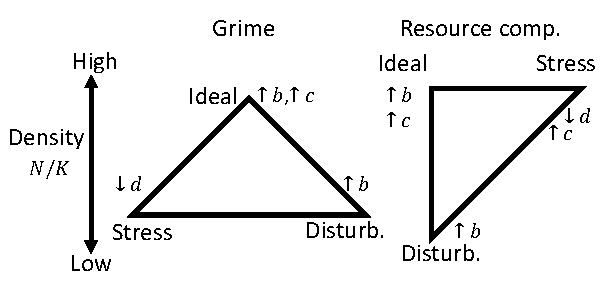
\includegraphics[scale=1]{axes.pdf}
\caption{\label{fig:axes} The realization of Grime's triangle in our model. Schematic representation of the triangular space bounded by the low/high extremes of stress/disturbance. The low-$T$ interpretation of stress is also shown. The vertices of the triangles correspond to environmental archetypes. Selection favors different traits at each vertex, leading to different trait clusters.} 
\end{figure}

How does Fig.~4 compare to Grime's C/S/R strategies? In our comparison we will stick to fishes, corals and plants, for which three-way primary strategy schemes are well developed \citep{grime_1977,winemiller_1992,darling_2012}. The connection of our model to fish strategies is necessarily more tentative, given that fishes are motile and not all territorial and the starting assumption of our model is site-occupancy . 

In disturbed environments, we predict evolution for higher $b$ and lower $d$, but not higher $c$. Higher $b$ means higher fecundity, but not necessarily mass propagule production: $b$ represents only those propagules which sucessfully develop into juveniles in unoccupied territories. This is broadly consistent with the ruderal primary strategy. Plant ruderals devote a large proportion of their productivity to seed production \cite{grime_1977}, whereas the analogous ``opportunistic'' strategists in fishes have large intrinsic growth rates \citep{winemiller_1992}. In corals, a distinguishing feature of the ruderal cluster is brood spawning (rather than broadcast spawning). This corresponds to higher parental investment and lower overall propagule production, but potentially also higher $b$ at low densities, since broadcast spawners are vulnerable to a powerful Allee effect at the egg fertilization stage \citep{knowlton_2001}. Lower $d$ could be achieved by improved individual resistance to physical destruction, but it is hard to reduce mortality in the face of severe disturbances. Given this constraint, shortening the time to reproductive maturity (the iteration time in our model) is an effective way of reducing the chance of death per iteration $d$. An exceptionally short life cycle is probably the most defining characteristic of ruderals \citep{grime_1977,winemiller_1992,darling_2012}.

In stressful environments, we predict evolution for lower $d$, and also  for higher $c$ in the low-$T$ interpretation of the stress archetype. Lowering $d$ is obviously essential when $b\ll 1$, and stress tolerant plants and corals have long life spans, allowing for long intervals between successful recruitments (and episodic broadcast spawning in corals). For fishes, the ``equilibrium'' strategy is the analogue of Grime's stress tolerator. This strategy is associated with resource limitation, and is also characterized by long life span, as well as high parental investment in tiny broods. This may reflect a high-$c$ strategy in the face of intense competition for severely limited resources (the low-$T$ interpretation).

In ideal environments, we predict evolution for higher $b$ and $c$, but not lower $d$. In plants and corals, a key mechanism for winning territorial contests is rapidly outgrowing and ``shading out'' competitors; not surprisingly, rapid individual growth is a defining feature of the competitor trait cluster \citep{grime_1977,darling_2012}. Evolution for higher $b$ under high-density, competitive conditions may seem counter-intuitive. Neither particularly high nor low $b$ have been associated with the competitor strategy in plants and corals. However, for fishes, the analogous ``periodic'' strategy is characterized by enormous brood sizes as well as rapid development \citep{winemiller_1992,winemiller_2015}, suggesting a strategy of ensuring that many propagules actually end up contesting areas favorable for development (higher $b$). The evolution of $b$ in ideal environments will be discussed further in the Discussion.

\section*{Discussion}

Unlike Grime's classic ternary plot \citep{grime_1974}, which represents anti-correlations between traits relevant for success in different environmental archetypes, our realization of Grime's triangle (Fig.~4) refers instead to the direction of trait evolution under different regimes of stress and disturbance. As discussed in section ``Primary strategies and Grime's triangle'', over time our predicted trait evolution should lead to trait values consistent with Grime's scheme. In making these predictions, we have made no reference to any kind of trade-offs or pleitropy, even though trade-offs are often invoked to explain primary strategy schemes \citep{macarthur_1962,winemiller_1992,aerts_1999}. Thus, while trade-offs may amplify specialization, they are not necessary for it. For example, corals which rapidly out-shade neighbors have a tall, branched morphology which is vulnerable to disturbances, and so, all else being equal, ideal environment $c$-strategists will suffer higher mortality from disturbances. Fig.~\ref{fig:axes} gives the same conclusion without invoking trade-offs; mutations which reduce disturbance vulnerability are essentially neutral under ideal conditions, leading to no improvements in mortality from disturbances, whereas $c$ will tend to increase over time. 

Our prediction of evolution for higher $b$ in ideal environments is counter to the expectations of MacArthur's $r$/$K$ dichotomy \citep{macarthur_1962} since $b$ is closely related to the maximal, low-density growth rate $b-d$, and ideal environments support high population densities which should be subject to ``$K$-selection''. However, in the Introduction, we noted that the $r$-$K$ dichotomy is not consistent with empirical studies showing that maximal growth rate and saturation density (measured by abundance) are positively correlated, both between species/strains \citep{luckinbill_1979,kuno_1991,hendriks_2005,fitzsimmons_2010}, and as a result of experimental evolution \citep{luckinbill_1978,luckinbill_1979}. From the perspective of our model, these correlations are not surprising since the saturation density, which is determined by a balance between births and deaths, increases with $b$. Our higher-$b$ prediction simply reflects the fact that, all else being equal, producing more propagules is always advantageous, regardless of population density, a fact lost in the simple logistic interpretation of the $r$/$K$ scheme. 

Confusingly, the term ``$K$-selection'' has sometimes been used to refer generally to selection at high density; this encompasses both selection for higher saturation density --- ``$K$'' in the logistic equation --- as well as selection for competitive ability. To avoid this ambiguity, the latter form of selection has been called ``$\alpha$-selection'' after the competition coefficients in the Lotka-Volterra equation \citep{gill_1974,case_1974,joshi_2001}. Unlike saturation density, there is support for a negative relationship between competitive success at high densities and maximal growth rate \cite{luckinbill_1979}; this could be driven by a tradeoff between individual size and reproductive rate. However, competitive success as measured by $\alpha$ (i.e. the per-capita effect of one genotype on another genotype's growth rate) is only partly determined by individual competitive ability --- in the presence of age-structure and territoriality, it also includes the ability of each genotype to produce contestants i.e. $b$ in our model. In contrast, our $c$ is strictly competitive ability only --- as such, it does not directly affect population density (section ``Model'').

$K$-selection in the sense of selection for a greater environmental carrying capacity for given birth and death rates, sometimes referred to as ``efficiency'' \citep{macarthur_1962}, would be represented in our model by smaller individual territorial requirements. To a first approximation, two co-occurring genotypes which differ by a small amount in their territorial requirements only should have the same fitness since the costs or benefits of a change in the amount of unocupied territory is shared equally among genotypes via the propagule density $L$. The situation is more complicated if those genotypes differ in multiple traits, and when the differences in territorial requirements become large enough that territorial contests can occur on different scales. We leave these complications for future work. 

The importance of $b$ in securing territories is a general feature of lottery competition. Indeed, as can be seen from Eq. \eqref{eq:lottery}, in the classic lottery model $b_i$ and $c_i$ are essentially equivalent in that only the products $b_i c_i$ matter \citep{chesson_1981}. This is no longer the case in our density-dependent generalization of the classic lottery model, where stable co-existence is possible between $b$ and $c$ strategists. Given that the classic lottery model was specifically developed for studying species co-existence questions, this may seem surprising, but the focus in that case was on the role of environmental fluctuations in promoting co-existence rather than stable coexistence \citep{chesson_1981}. It is not clear whether correctly accounting for the behavior of species with low density would significantly alter the conclusions of \cite{chesson_1981}, but, in any case, species co-existence questions are beyond the scope of this manuscript. 

More broadly, while our model can be applied to questions at a species level (e.g. ecological invasions), our focus here is on the evolution of genotype frequencies within a population. This is only possible because the model accounts for the growth of mutants from low densities. Given this focus, our assumption that there are no large $c$ discrepancies (section ``Mean field approximation'') amounts to a restriction on the amount of genetic variation in $c$ that will be sustained in the population. Since beneficial mutation effect sizes will typically not be much larger than a few percent, large $c$ discrepancies can only arise if the mutation rate is extremely large, and so the assumption will not be violated in most cases. However, this restriction could become important when looking at species interactions rather than genotype evolution.

In our view, the density dependent lottery model has two major limitations as a general-purpose model of density-dependent selection: a reliance on interference competition for durable resources (territoriality), and the restriction of competition to juveniles (lottery recruitment to adulthood). In some respects this is the complement of resource competition models, which restrict their attention to exploitation competition, typically without age structure \citep{tilman_1982}. In the particular case that resources are spatially localized (e.g. due to restricted movement through soils), then resource competition and territorial acquisition effectively coincide, and in principle a competitive ability $c$ should be derivable from resource competition. The situation is more complicated if the resources are well-mixed, since, in general, resource levels then need to be explicitly tracked. It is possible that explicit resource tracking is in fact not necessary when the focus is on the evolution of similar genotypes rather than the stable co-existence of widely differing species. We are not aware of any attempts to delineate the conditions under which explicit resource tracking is not required, let alone to connect those results to the density-dependent selection literature [need to check Tilman's book]. 

On the other hand, the model does remarkably well in capturing apparently general features of selection under different environmental conditions using only three trait parameters: $b$, $c$ and $d$. The clean separation of a strictly-relative $c$ parameter is particularly useful from an evolutionary genetics perspective, essentially embedding a relative fitness trait within an absolute fitness model. This could have interesting applications for modeling the impacts of intra-specific competition on species extinction, without arbitrarily assigning an absolute fitness cost to that competition. [citations to sexual selection stuff?]

\bibliographystyle{amnatnat}
\bibliography{reference} 

\section*{Appendix A: Poisson approximation}

The propagule numbers $x_i$ in different territories are not independent random variables. To determine the dispersal outcomes in all unoccupied territories exactly, we would need to proceed territory-by-territory as follows. In the first territory we evaluate, $x_i$ drawn from a binomial distribution with $m_i$ trials and success probability $1/U$. In the second, $x_i$ is drawn from a binomial distribution with $m_i-x$ trials and success probability $1/(U-1)$, where $x$ is the number of propagules that landed in the first territory. And so on.

For sufficiently large $K$, holding $n_i/T$ fixed, the Poisson limit theorem implies that the binomial distributions for $x_i$ at each successive stage of this procedure are all closely approximated by a Poisson distribution with mean $l_i$, where we have used the fact that large $T$ implies large $U$ except in the biologically uninteresting case that there is vanishing population turnover $d_i \sim 1/T$. 

Under the Poisson approximation, the total number of genotype $i$ propagules $\sum x_i$ (summed over unoccupied territories) will deviate about its mean value $m_i$. Since the coefficient of variation of $\sum x_i$ is proportional to $1/\sqrt{m_i}$, these deviations are negligible unless $m_i$ is very small (say of order $10^2$ or less).

\section*{Appendix B: Derivation of growth equation}

We separate the right hand side of Eq.~\eqref{eq:growthsumuncoupled} into three components $\Delta_+ n_i = \Delta_u n_i+\Delta_r n_i+\Delta_a n_i$ which vary in relative magnitude depending on the propagule densities $l_i$. Following the notation in the main text, the Poisson distributions for the $x_i$ (or some subset of the $x_i$) will be denoted $p$, and we use $P$ as a general shorthand for the probability of particular outcomes.

\subsection*{Growth without competition}

The first component, $\Delta_u n_i$, accounts for territories where only one focal propagule is present $x_i=1$ and $x_j=0$ for $j\neq i$ ($u$ stands for ``uncontested''). The proportion of territories where this occurs is $l_i e^{-L}$, and so 
\begin{equation}
\Delta_u n_i=Ul_i e^{-L}=m_i e^{-L}.
\end{equation}

\subsection*{Competition when rare}

The second component, $\Delta_r n_i$, accounts for territories where a single focal genotype propagule is present along with at least one non-focal propagule ($r$ stands for ``rare'') i.e. $x_i=1$ and $\sum_{j\neq i} x_j\geq 1$. The number of territories where this occurs is $Up_i(1)P(\sum_{j\neq i} x_j\geq 1)=b_i n_i e^{-l_i}(1-e^{-(L-l_i)})$. Thus 
\begin{equation}
\Delta_r n_i = m_i e^{-l_i}(1-e^{-(L-l_i)})\left\langle  \frac{c_i}{c_i +\sum_{j\neq i} c_j x_j } \right\rangle_{\tilde{p}},  \label{eq:deltr}
\end{equation}
where $\langle \rangle_{\tilde{p}}$ denotes the expectation with respect to $\tilde{p}$, and $\tilde{p}$ is the probability distribution of nonfocal propagule abundances $x_j$ \textit{after} dispersal, in those territories where exactly one focal propagule, and at least one non-focal propagule, landed. 

We now show that, with respect to $\tilde{p}$, the standard deviation $\sigma_{\tilde{p}}(\sum_{j\neq i} c_j x_j)$, is much smaller than its mean $\langle\sum_{j\neq i} c_j x_j\rangle_{\tilde{p}}$. Then $x_j$ can be replaced by its mean in the last term in Eq.~\eqref{eq:deltr},
\begin{equation}
\left\langle\frac{c_i}{c_i +\sum_{j\neq i} c_j x_j}\right\rangle_{\tilde{p}}\approx \frac{c_i}{c_i +\sum_{j\neq i} c_j \langle x_j\rangle_{\tilde{p}}}.\label{eq:meanfieldr}
\end{equation}

The exact expression for $\langle x_j \rangle_{\tilde{p}}$ is somewhat complicated. Let $X$ denote the total number of propagules in a territory,  ${\mathbf x_i}=(x_1,\ldots,x_{i-1},x_{i+1}\ldots,x_G)$ denote the vector of non-focal abundances, so that $p({\mathbf x_i})=p_1(x_1)\ldots p_{i-1}(x_{i-1})p_{i+1}(x_{i+1})\ldots p_G(x_G)$, and let $X_i=X-x_i$ denote the total number of nonfocal propagules. Then, $\tilde{p}$ can be written as
\begin{align}
\tilde{p}({\mathbf x_i})&=p({\mathbf x_i}|X\geq 2,x_i=1)\nonumber\\
&=\frac{P({\mathbf x_i},X\geq 2|x_i=1)}{P(X\geq 2)}\nonumber\\
&=\frac{1}{1-(1+L)e^{-L}}\sum_{k=2}^{\infty} P(k) p({\mathbf x_i}|X_i=k-1),
\end{align}
and so
\begin{align}
\langle x_j \rangle_{\tilde{p}}&=\sum_{\mathbf x_i} \tilde{p}({\mathbf x_i})x_j,\nonumber\\
&=\frac{1}{1-(1+L)e^{-L}}\sum_{k=2}^{\infty} P(k) \sum_{\mathbf x_i} p({\mathbf x_i}|X_i=k-1)x_j.
\label{eq:raremonster1}
\end{align}
The inner sum over ${\mathbf x_i}$ is the mean number of $j$ propagules that will be found in a territory which received $k-1$ nonfocal propagules, which is equal to $\frac{l_j}{L-l_j}(k-1)$. Thus, 
\begin{align}
\langle x_j \rangle_{\tilde{p}}&=\frac{l_j}{1-(1+L)e^{-L}}\frac{1}{L-l_i}\sum_{k=2}^{\infty} P(k) (k-1),\nonumber\\
&=\frac{l_j}{1-(1+L)e^{-L}}\frac{L-1+e^{-L}}{L-l_i},
\label{eq:meanxjrare}
\end{align}
where the last line follows from the fact that $\sum_{k=2}^{\infty} P(k)(k-1)=\sum_{k=1}^{\infty} P(k)(k-1)=\sum_{k=1}^{\infty} P(k)k-\sum_{k=1}^{\infty}P(k)=L-(1-e^{-L})$.

For analyzing the relative fluctuations in $\sum_{j\neq i} c_j x_j$, Eq. \eqref{eq:meanxjrare} is unnecessarily complicated, and so we instead use the following approximation. Rather than evaluating the situation in each territory after dispersal as above, we replace $\tilde{p}$ by $\tilde{q}$, defined as the ${\mathbf x_i}$ dispersal probabilities, conditional on $X_i>1$, in a territory where one focal propagule is assumed to already be present. This gives $\langle x_j \rangle_{\tilde{q}}=l_j/C$, 
\begin{equation}
\sigma_{\tilde{q}}^2(x_j)=\frac{l_j^2}{C}\left(1-\frac{1}{C}\right)+\frac{l_j}{C},\label{eq:varr}
\end{equation}
and 
\begin{equation}
\sigma_{\tilde{q}}(x_j,x_k)=\frac{l_j l_k}{C}\left(1-\frac{1}{C}\right),\label{eq:covr}
\end{equation}
where $C=1-e^{-(L-l_i)}$. Comparing $\langle x_j \rangle_{\tilde{q}}=l_j/C$ and Eq.~\eqref{eq:meanxjrare}, the subtle difference in how we defined $\tilde{q}$ leads to considerably simpler expressions for the mean of $x_j$ (similarly for variances and covariances of the $x_j$, which we did not have the courage to calculate with $\tilde{p}$). To be sure, $\tilde{q}$ is incorrect: assuming that one propagule is already present biases total number of propagules by one. For example, if the focal genotype is rare and the propagule density is high ($l_j \approx L\gg 1$), Eq. \eqref{eq:meanxjrare} correctly gives $\langle x_j \rangle_{\tilde{p}}\approx L-1$, whereas $\langle x_j \rangle_{\tilde{q}}\approx L$. As a result, $\tilde{q}$ leads to pathological behavior for rare invaders (they have a rarity disadvantage), but its moments are quantitatively similar enough to $\tilde{p}$'s that it is sufficient for analyzing the relative fluctuations in $\sum_{j\neq i} c_j x_j$.

Decomposing the variance in $\sum_{j\neq i} c_j x_j$,
\begin{equation}
\sigma_{\tilde{q}}^2(\sum_{j\neq i} c_j x_j)=\sum_{j\neq i}\left[c_j^2\sigma_{\tilde{q}}^2(x_j)+2\sum_{k>j}c_j c_k\sigma_{\tilde{q}}(x_j,x_k)\right],\label{eq:vartotr}
\end{equation}
and using the fact that $1/C>1$ which implies that the first term in Eq. \eqref{eq:varr} and $\sigma_{\tilde{q}}(x_j,x_k)$ are negative, the relative fluctuations in $\sum_{j\neq i} c_j x_j$ satisfy
\begin{equation}
\frac{\sigma(\sum_{j\neq i} c_j x_j)}{\langle\sum_{j\neq i} c_j x_j\rangle}<C^{1/2}\frac{\left(\sum_{j\neq i}c_j^2 l_j\right)^{1/2}}{\sum_{j\neq i}c_j l_j}. \label{eq:cvr}
\end{equation}

Without loss of generality, we restrict attention to the case that the total nonfocal density $L-l_i$ is of order $1$ or larger (otherwise $\Delta_r n_i$ does not contribute significantly to $\Delta_+ n_i$ because $\Delta_r n_i$ is proportional to $C=1-e^{-(L-l_i)}$).

When at least some of the nonfocal propagule densities are large $l_j\gg 1$, then the RHS of Eq.~\eqref{eq:cvr} is $\ll 1$, as desired. This is also the case if none of the nonfocal genotype densities are large and the $c_j$ are all of similar magnitude (their ratios are of order one); the worst case scenario occurs when $(L-l_i)\sim O(1)$, in which case the negative covariances (Eq.~\eqref{eq:covr}) which were neglected in the RHS of Eq.~\eqref{eq:cvr} significantly reduce the overall variance $\sigma_{\tilde{q}}^2(\sum_{j\neq i} c_j x_j)$.

However, the relative fluctuations in $\sum_{j\neq i} c_j x_j$ can be large if some of the $c_j$ are much larger than the others. Specifically, if $c_j l_j\gg c_k l_k$ ($j,k\neq i$; $j\neq k$) and $l_j\ll 1$ (i.e. in the presence of a rare, extremely strong competitor), then we cannot make the replacement Eq.~\eqref{eq:meanfieldr}. 

Substituting Eqs. \eqref{eq:meanfieldr} and \eqref{eq:meanxjrare} into Eq.~\eqref{eq:deltr}, we obtain
\begin{equation}
\Delta_r n_i\approx m_i R_i\frac{c_i}{\overline{c}}, \label{eq:deltrfinal}
\end{equation}
where $R_i$ is defined in Eq.~\eqref{eq:Dr}.

\subsection*{Competition when abundant}

The final contribution, $\Delta_a n_i$, accounts for territories where two or more focal propagules are present ($a$ stands for ``abundant"). Similarly to Eq.~\eqref{eq:deltr}, we have 
\begin{equation}
\Delta_a n_i=U(1-(1+l_i)e^{l_i})\left\langle \frac{c_i x_i}{\sum_j c_j x_j} \right\rangle_{\hat{p}}\label{eq:delta}
\end{equation}
where $\hat{p}$ is the probability distribution of both focal and nonfocal propagaule abundances \textit{after} dispersal in those territories where at least two focal propagules landed. 

Again, we show that the relative fluctuations in $\sum c_j x_j$ are much smaller than $1$ (with respect to $\hat{p}$), so that we have 
\begin{equation}
\left\langle \frac{c_i x_i}{\sum_j c_j x_j} \right\rangle_{\hat{p}}\approx  \frac{c_i \langle x_i \rangle_{\hat{p}}}{\sum_j c_j \langle x_j\rangle_{\hat{p}}}.\label{eq:meanfielda}
\end{equation}
Following a similar procedure as for $\Delta_r n_i$, where the vector of propagule abundances is denoted ${\mathbf x}$, we have
\begin{align}
\langle x_j \rangle_{\hat{p}}&=\sum_{\mathbf x} x_j p(\mathbf x|x_i\geq 2)\nonumber \\
&=\sum_{k}P(k|x_i\geq 2)\sum_{\mathbf x} x_j p({\mathbf x}|x_i\geq 2,k)\nonumber\\
&=\sum_{k}P(k|x_i\geq 2)\sum_{x_i} \sum_{\mathbf x_i} x_j p(\mathbf x_i|\sum_{j\neq i} x_j=k-x_i)p(x_i|x_i\geq 2,k)\nonumber\\
&=\sum_{k}P(k|x_i\geq 2)\sum_{x_i} \frac{l_j(k-x_i)}{L-l_j} p(x_i|x_i\geq 2,k)\nonumber\\
&=\frac{l_j}{L-l_j}\left( L\frac{1-e^{-L}}{1-(1+L)e^{-L}}- l_j\frac{1-e^{-l_j}}{1-(1+l_j)e^{-l_j}}\right) 
\end{align}
for $j\neq i$, and 
\begin{equation}
\langle x_i\rangle_{\hat{p}}=l_i\frac{1-e^{-l_i}}{1-(1+l_i)e^{-l_i}}.
\end{equation}

To calculate the relative fluctuations in $\sum_{j\neq i} c_j x_j$, we use a similar approximation as for $\Delta_r n_i$: $\hat{p}$ is approximated by the ${\mathbf x}$ dispersal probabilities in a territory where at least two focal propagule is assumed to be present. All covariances are now zero, so that $\sigma^2(\sum c_j x_j)=\sum c_j^2 \sigma^2(x_j)$, where $\sigma^2(x_j)=l_j$ for $j\neq i$. The expression for $\sigma^2(x_i)$ is more complicated. We assume $p(x_i=0)\approx 0$ without loss of generality (since otherwise $D\gg 1$ and $\Delta n_a$ is negligible). Then
\begin{equation}
\sigma^2(x_i)=\frac{l_i^2}{D}\left(1-\frac{1}{D}\right)+\frac{l_i}{D},
\end{equation}
where $D=1-(1+l_i)e^{-l_i}$, analogous to Eq.~\eqref{eq:varr}, and 
\begin{equation}
\frac{\sigma(\sum c_j x_j)}{\langle\sum c_j x_j\rangle} \approx\frac{\left(\sum_{j\neq i} c_j^2 l_j + c_i^2 \sigma^2(x_i)\right)^{1/2}}{\sum_{j\neq i} c_j l_j + c_i l_i/D} \label{eq:cva}.
\end{equation}

Similarly to Eq.~\eqref{eq:cvr}, the RHS of \eqref{eq:cva} will not be $\ll1$ if there is a nonfocal genotype $j$ with $l_j\ll 1$ and $c_j l_j\gg c_k l_k$ for $j,k\neq i$, $j\neq k$. When this is not the case, then since $l_i$ must be of order $1$ or larger for $\Delta_a n$ to make an appreciable contribution to $\Delta_+ n_i$, the RHS of Eq.~\eqref{eq:cva} is $\ll 1$ as desired. 

Combining Eqs. \eqref{eq:delta} and \eqref{eq:meanfielda}, we obtain
\begin{equation}
\Delta_a n_i=m_i A_i \frac{c_i}{\overline{c}},
\end{equation}
where $A_i$ is defined in Eq.~\eqref{eq:Da}.

%The logistic equation for a single genotype or species is given by
%\begin{equation}
%\frac{dN}{dt}=r\left(1-\frac{N}{K}\right)N \label{eq:logistic}
%\end{equation}
%where $N$ is the total population abundance or biomass, $r$ is the growth rate at  low densities, and the ``carrying capacity" $K$ is the value of $N$ where growth ceases.
%
%a simple, ubiquitous model of density-dependent population growth
%declines linearly with density,
%
%Eq.~\eqref{eq:logistic} is often interpreted as a linear approximation of a more complicated growth equation
%\begin{equation}
%\frac{dN}{dt}=r(N)N,
%\end{equation}
%where the growth rate $r(N)$ is some unknown, possibly complicated, function of $N$. 

%\subsection{Logistic growth and classic nesting sites model}

%In the nesting sites model, it is assumed that propagules landing on occupied territory do not survive, while those landing on unoccupied territory immediately occupy the territory. Thus, the probability that a propagule survives is simply $(1-N/K)$, where $N=\sum_i n_i$ is the total population size. Consequently, $n_i$ increases by $1$ over the interval $[t,t+\Delta t]$ with probability $b_i n_i (1-N/K)\Delta t$. Provided that the abundances $n_i$ are large enough that demographic stochasticity is negligible (i.e. they have established), we can treat $n_i(t)$ as a continuous variable with growth given by the expectation of $b_i n_i (1-N/K)\Delta t$, and so, taking $\Delta t \rightarrow 0$ we obtain
%\begin{equation}
%\frac{dn_i}{dt}=b_i\left(1-\frac{N}{K}\right)n_i. \label{eq:logistic}
%\end{equation}

%\section{Territorial availability}
%
%In Sec. \ref{sec:c} we assumed that adults have the same territorial requirement, regardless of genotype. This can be generalized to allow genotypes to differ in their territorial requirements. Each adult from genotype $i$ now requires $t_i$ units of territory, $T$ is the total territory available to the population, and $T-\sum_i t_i$ units of territory are unoccupied. 
%
%Competition between propagules with different territorial requirements is potentially much more complicated than the model in Sec. \ref{sec:c}, because competition is no longer neatly partitioned into a set of identical territories.  The larger a propagule's territorial requirement, the more neighboring propagules it will interact with during its development to adulthood. 
%
%
%A simple way to avoid these complications is to partition the unoccupied territory into uniform units of territory with size given by the largest territorial requirement $t^*={\rm max}_i t_i$. The uniform territory approach used in Sec.  \ref{sec:c}
%
%The biological intuition behind this 
%
%Thus $U=(T-\sum_i t_i n_i)/t^*$.


\end{document}
